\documentclass[10pt,letter,twoside]{article}
\usepackage[utf8]{inputenc}
\usepackage{amsmath}
\usepackage{amsfonts}
\usepackage{amssymb}
\usepackage[spanish,es-noshorthands]{babel}
\usepackage[T1]{fontenc}
\usepackage{lmodern}
\usepackage{graphicx,hyperref}
\usepackage{tikz,pgf}
\usepackage{multicol}
\usepackage{subfig}
\usepackage[width=7.5in,height=9.5in]{geometry}
\usepackage{fancyhdr}
\pagestyle{fancy}
\usepackage{marvosym}
\fancyhead[LE]{\url{https://www.autistici.org/mathgerman}}
\fancyhead[RE]{}
\fancyhead[RO]{}
\fancyhead[LO]{}
\fancyfoot[LE,RO]{\Email~ iedabgerman@autistici.org}
\fancyfoot[CE,CO]{\thepage}
\author{Germ\'an Avenda\~no Ram\'irez~\thanks{Lic. U.D., M.Sc. U.N.}}
\title{\begin{minipage}{.2\textwidth}

\includegraphics[height=1.75cm]{Images/logo-colegio.png}\end{minipage}
\begin{minipage}{.55\textwidth}
\begin{center}
Taller 2, Números reales\\
Cálculo $11^{\circ}$
\end{center}
\end{minipage}\hfill
\begin{minipage}{.2\textwidth}

\includegraphics[height=1.75cm]{Images/logo-sed.png} 
\end{minipage}}
\date{}
\thispagestyle{plain}
\begin{document}
\maketitle
Nombre: \hrulefill Curso: \underline{\hspace*{44pt}} Fecha: \underline{\hspace*{2.5cm}}\\
\begin{multicols}{2}
\section*{Números reales}
\begin{enumerate}
  \item La oficina postal solamente aceptará paquetes cuya longitud más su grueso (distancia alrededor), no supere las 108 pulgadas.	Luego, para el paquete de la figura tenemos que:
  \[L+2(x+y)\leq108 \]
  \begin{enumerate}
   \item ¿Aceptará la oficina postal un paquete que tiene 6 pulgadas de ancho, 8 pulgadas de fondo y 5 pies de largo? ¿Y un paquete que mide 2  pies por 2 pies por 4 pies?
   \item ¿Cuál es la mayor longitud que puede tener un paquete para ser aceptado que tiene una base cuadrada de 9 pulgadas por 9 pulgadas?.
  \end{enumerate}
  \begin{center}
 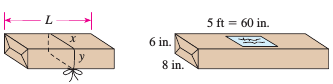
\includegraphics[scale=.9]{./Images/paquetepostal.png}
 % paquetepostal.png: 0x0 pixel, 300dpi, 0.00x0.00 cm, bb=
\end{center}
\item \emph{Signo de los números}: Sean $a$, $b$ y $c$ números reales con $a>0$, $b<0$ y $c<0$. Encuentre el signo de cada expresión.
\begin{enumerate}
\begin{multicols}{3}
 \item $-a$
 \item $-b$
 \item $bc$
 \item $a-b$
 \item $c-a$
 \item $a+bc$
 \item $ab+ac$
 \item $-abc$
 \item $ab^{2}$
 \end{multicols}
\end{enumerate}
\item Explique por qué la suma, la diferencia, y el producto de dos números racionales es otro número racional. ¿Es el producto de dos números irracionales necesariamente un número irracional? ¿Y la suma?
\item \textbf{Combinando n\'{u}meros racionales con n\'umeros irracionales}: ¿Es $\frac{1}{2}+\sqrt{2}$ racional o irracional? ¿Es $\frac{1}{2}\cdot \sqrt{2}$ racional o irracional?
 En general, que puede decir acerca de la suma de un n\'umero racional y un n\'umero irracional? ¿Y del producto?
 \item \textbf{Números irracionales y geometría:} Unando la siguiente figura, explique como localizar el punto $\sqrt{2}$ en la recta numérica. ¿Puede localizar el número $\sqrt{5}$ con un método similar? ¿Y $\sqrt{6}$? Muestre otros números irracionales que pueden ser ubicados así.
 \begin{center}
 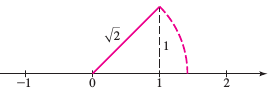
\includegraphics{./Images/raizde2.png}
 % raizde2.png: 0x0 pixel, 300dpi, 0.00x0.00 cm, bb=
\end{center}
\item Sabemos que la adición y la multiplicación son ambas operaciones conmutativas.
\begin{enumerate}
 \item ¿Es la sustracción conmutativa?
 \item ¿Es la división por un número real diferente de 0 una operación conmutativa?
\end{enumerate}
\item Escriba cada expresión radical usando exponentes, y, cada expresión con exponentes, usando radicales:
\begin{center}
\begin{tabular}{|c|c|}\hline
Expresión radical & Expresión con exponentes\\ \hline
$\dfrac{1}{\sqrt{5}}$ & \rule[-0.3cm]{0cm}{0.8cm}\\ \hline
$\sqrt[3]{7^{2}}$ & \rule[-0.3cm]{0cm}{0.8cm}\\ \hline
 & $4^{\frac{2}{3}}$\rule[-0.3cm]{0cm}{0.8cm}\\ \hline
 & $11^{-\frac{3}{2}}$\rule[-0.3cm]{0cm}{0.8cm}\\ \hline
$\sqrt[5]{5^{3}}$ & \rule[-0.3cm]{0cm}{0.8cm}\\ \hline
 & $2^{-15}$\rule[-0.3cm]{0cm}{0.8cm}\\ \hline
 & $a^{\frac{2}{5}}$\rule[-0.3cm]{0cm}{0.8cm}\\ \hline
$\dfrac{1}{\sqrt{x^{5}}}$ & \rule[-0.3cm]{0cm}{0.8cm}\\\hline
\end{tabular}
\end{center}
~\ref{num:9}--\ref{num:18} Evalúe cada expresión
\item \label{num:9}
 \begin{enumerate}\begin{multicols}{3}
 \item $-3^{2}$
 \item $(-3)^{2}$
 \item $(-3)^{0}$
 \end{multicols}
 \end{enumerate}
 \item 
 \begin{enumerate}
 \begin{multicols}{3}
 \item $5^{2}(\frac{1}{5})^{3}$
 \item $\dfrac{10^{7}}{10^{4}}$
 \item $\dfrac{3}{3^{-2}}$
 \end{multicols} 
 \end{enumerate}
 \item 
 \begin{enumerate}\begin{multicols}{3}
  \item $\dfrac{4^{-3}}{2^{-8}}$
  \item $\dfrac{3^{-2}}{9}$
  \item $(\frac{1}{4})^{-2}$
  \end{multicols}
 \end{enumerate}
\item 
\begin{enumerate}\begin{multicols}{3}
 \item $(\frac{2}{3})^{-3}$
 \item $(\frac{3}{2})^{-2}\cdot \frac{9}{16}$
 \item $(\frac{1}{2})^{4}\cdot (\frac{5}{2})^{-2}$
 \end{multicols}
\end{enumerate}
\item 
\begin{enumerate}\begin{multicols}{3}
 \item $\sqrt{16}$
 \item $\sqrt[4]{16}$
 \item $\sqrt[4]{\frac{1}{16}}$
 \end{multicols}
\end{enumerate}
\item 
\begin{enumerate}\begin{multicols}{3}
 \item $\sqrt{64}$
 \item $\sqrt[3]{-64}$
 \item $\sqrt[5]{-32}$
 \end{multicols}
\end{enumerate}
\item 
\begin{enumerate}\begin{multicols}{3}
 \item $\sqrt[3]{\dfrac{8}{27}}$
\item $\sqrt[3]{\dfrac{-1}{64}}$
\item $\dfrac{\sqrt[5]{-3}}{\sqrt[5]{96}}$ 
 \end{multicols}
\end{enumerate}
\item 
\begin{enumerate}\begin{multicols}{3}
 \item $\sqrt{7}\sqrt{28}$
 \item $\dfrac{\sqrt{48}}{\sqrt{3}}$
 \item $\sqrt[4]{24}\sqrt[4]{54}$
 \end{multicols}
\end{enumerate}
\item 
\begin{enumerate}\begin{multicols}{3}
 \item $(\frac{4}{9})^{-1/2}$
 \item $(-32)^{2/5}$
 \item $-32^{2/5}$
 \end{multicols}
\end{enumerate}
\item \label{num:18}
\begin{enumerate}\begin{multicols}{3}
 \item $1024^{-0.1}$
 \item $(-\frac{27}{8})^{2/3}$
 \item $(\frac{25}{64})^{-3/2}$
 \end{multicols}
\end{enumerate}
~\ref{num:19}--\ref{num:22} Evalúe las expresiones, si $x=3$, $y=4$, y, \\$z=-1$\\
\begin{multicols}{2}
\item \label{num:19} $\sqrt{x^{2}+y^{2}}$
\item $\sqrt[4]{x^{3}+14y+2z}$
\item $(9x)^{2/3}+(2y)^{2/3}+z^{2/3}$
\item \label{num:22} $(xy)^{2z}$
\end{multicols}
\ref{num:23}--\ref{num:26} Simplifique las expresiones
\begin{multicols}{2}
\item \label{num:23} $\sqrt{32}+\sqrt{18}$
\item $\sqrt{75}+\sqrt{48}$
\item $\sqrt[5]{96}+\sqrt[5]{3}$
\item \label{num:26} $\sqrt[4]{48}-\sqrt[4]{3}$
\end{multicols}
\ref{num:27}--\ref{num:44} Simplifique la expresión y elimine cualquier exponente negativo
\begin{multicols}{2}
\item \label{num:27} $a^{9}a^{-5}$
\item $(3y^{2})(4y^{5})$
\item $(12x^{2}y^{4})(\frac{1}{2}x^{5}y)$
\item $(6y)^{3}$
\item $\dfrac{x^{9}(2x)^{4}}{x^{3}}$
\item \label{num:44} $\dfrac{a^{-3}b^{4}}{a^{-5}b^{5}}$
\end{multicols}
\item Calcula y simplifica
\begin{enumerate}\begin{multicols}{2}
  \item $ \sqrt{12}-\sqrt{48}+\sqrt{27} $  
  \item $ \sqrt[3]{24}-\sqrt[3]{375}+\sqrt[3]{81} $
\end{multicols}
\end{enumerate}
\item Calcula y simplifica
\begin{enumerate}\begin{multicols}{2}
  \item $ (\sqrt{5}+\sqrt{2})^2 $  \item $ (2\sqrt{5}+\sqrt{3})^2 $ \item $ (\sqrt{3}-\sqrt{2})(2-\sqrt{2}) $
\end{multicols}
\end{enumerate}
\item Calcula y simplifica
\begin{enumerate}\begin{multicols}{3}
  \item  $ \sqrt{\frac{7}{5}}\sqrt{35} $
  \item $ \sqrt{\frac{3}{2}}\sqrt{\frac{8}{3}} $
  \item $ \sqrt{\frac{10}{3}}\sqrt{7,5}$
\end{multicols}
\end{enumerate}
\item Dibuja un cuadrado de 5 cm de lado. Dibuja otro cuadrado que tenga doble área.
\item Dibuja un rectángulo cuya diagonal valga 5
\item Las dimensiones de una aula son 12 m de largo, 7 m de ancho y 3,40 m de alto. Dos moscas revoletean por el aula. ¿Cuál es la distancia máxima a que pueden encontrarse?
\item Representa:
\begin{enumerate}
\begin{multicols}{2}
 \item $ [4,6]\cup (9,11)$
 \item $ [-6,5]\cap (2,5) $
 \item $ (2,7)\cap (5,9)\cap (6,10) $
  \end{multicols}
\end{enumerate}
  \item Calcula:
  \begin{enumerate}\begin{multicols}{2}
    \item $ \sqrt{1024} $    \item $ \sqrt{441} $
    \item $ \sqrt[3]{729} $ \item $ \sqrt[4]{1296} $
    \item $ \sqrt[5]{-1} $ \item $ 28-2\sqrt{81} $
    \item $ \sqrt{4+2\cdot16} $
    \item $ 8+2\sqrt[3]{-8} $ \item $ \sqrt{400-16-60} $
    \item $ \sqrt{5+\sqrt{13\sqrt{9}}} $
    \item $ \sqrt{10+2\sqrt{7+\sqrt[3]{8}}} $
    \item $ \sqrt{4,7+1,06} $
    \item $ 3\sqrt[3]{0,001+2} $ \item $ \sqrt[4]{\frac{1}{625}} $
    \item $ \sqrt[5]{\frac{-1}{32}} $ \item $ \sqrt{\frac{1}{4}}-\sqrt{\frac{9}{25}} $ \item $ \sqrt{\frac{9}{4}\div \sqrt{\frac{121}{25}}} $
  \end{multicols}
  \end{enumerate}
  \item Calcula
  \begin{enumerate}
    \item $ \left(\sqrt{5+\sqrt{5}}\right)\left(\sqrt{5-\sqrt{2}}\right) $
    \item $ (2+\sqrt{3})^2 $
    \item $ (1+\sqrt{2})(1+\sqrt{2})\sqrt{2} $
  \end{enumerate}
  \item Transforma en radicales
  \begin{enumerate}\begin{multicols}{4}
    \item $ (-3)^{\frac{1}{5}} $  \item $ \left(\frac{3}{5}\right)^{3/7} $  \item $ \left(\frac{2}{3}\right)^{-3/2} $
    \item $ \left(\frac{1}{5}\right)^{-1/4} $
  \end{multicols}
  \end{enumerate}
  \item Halla usando la calculadora
  \[ \sqrt[5]{12^3}\qquad \dfrac{1}{\sqrt[7]{7^4}}\qquad \sqrt[3]{11^2} \]
  \item Encuentra todos los números de tres cifras que sean cubos de un número natural
  \item En la descomposición de cierta cantidad de agua por electrólisis, se obtienen 2 litros de hidrógeno y 16 litros de oxígeno ¿Cuál es la producción de hidrógeno? ¿Y de oxígeno? Expresa los resultados en tanto por ciento. ¿Qué cantidad de oxígeno se obtendrán con 54 litros de agua?
  \item ¿Cuántas baldosas cuadradas de 20 cm de lado se necesitan para recubrir una superficie de 27,04 $ m^2 $?
  \item Halla la arista de un cubo cuyo volumen es 46,656 $m^3$.
  \item Un depósito cúbico tiene una capacidad de 157.464 litros. ¿Cuál es la superficie de cada una de las paredes del deposito?
\end{enumerate}
\end{multicols}
\end{document}
